\documentclass{article}

\usepackage[utf8]{inputenc}

\usepackage{graphicx}
\usepackage{subcaption}
\usepackage{mathtools}
\usepackage{wrapfig}
\usepackage{graphicx}
\usepackage{subcaption}
\usepackage{mathtools}
\usepackage{wrapfig}
\usepackage{float}
\usepackage{gensymb}
\usepackage{caption}
\usepackage{geometry}
\usepackage{cite}

\DeclareMathOperator{\sech}{sech}
\DeclareMathOperator{\Tr}{Tr}

\usepackage{listings}
\usepackage{color}

\definecolor{codegreen}{rgb}{0,0.6,0}
\definecolor{codegray}{rgb}{0.5,0.5,0.5}
\definecolor{codepurple}{rgb}{0.58,0,0.82}
\definecolor{backcolour}{rgb}{0.95,0.95,0.92}
 
\lstdefinestyle{mystyle}{
    backgroundcolor=\color{backcolour},   
    commentstyle=\color{codegreen},
    keywordstyle=\color{magenta},
    numberstyle=\tiny\color{codegray},
    stringstyle=\color{codepurple},
    basicstyle=\footnotesize,
    breakatwhitespace=false,         
    breaklines=true,                 
    captionpos=b,                    
    keepspaces=true,                 
    numbers=left,                    
    numbersep=5pt,                  
    showspaces=false,                
    showstringspaces=false,
    showtabs=false,                  
    tabsize=2
}
 
\lstset{style=mystyle}




\makeatletter
\renewcommand\paragraph{\@startsection{paragraph}{4}{\z@}%
	{-2.5ex\@plus -1ex \@minus -.25ex}%
	{1.25ex \@plus .25ex}%
	{\normalfont\normalsize\bfseries}}
\makeatother
\setcounter{secnumdepth}{4} % how many sectioning levels to assign numbers to
\setcounter{tocdepth}{4}    % how many sectioning levels to show in ToC in preamble





\geometry
{
  %body={6.5in, 8.5in},
  left=1.0in,
  top=1.25in
}

\setlength{\parindent}{10ex}




%\begin{figure}[H]
%	\centering
%	\includegraphics[scale=0.2]{rhul_logo}
%\end{figure}

%questions for chris
%is there a paper for the creation of InterDyne that can be referenced, or is the webpage all there is? ref webpage

%why do we need simple models of the finical markets, used to build the tools and methods that can then be used to analyse complex models/real fincial markets

%when to use et al , should i say clack and students [refrences]

%feedback loops that always return the same value, no dependces therefore not part of a loop 

%use the line "the work this paper is built on", interdyne project, creators or interdyne 

\begin{document} 
\title{Defining the Semantics of Agent Based Modelling in InterDyne}
\author{Leo Carlos-Sandberg\\
Supervisor: Dr Christopher D. Clack} 
\maketitle 

\begin{abstract}
\noindent {\it This paper defines the semantics of agent based modelling within the Interdyne simulator. A converter has been created that links an agent based model step wise to a difference equation based language, this language is created in such a way that it is directly relatable to lambda calculus which can then be used as definition of the semantics of the agent based model.
%talk about this helping regulators 
}
\end{abstract}




\newpage
\newgeometry{top = 2cm}
\tableofcontents
{\textit{ }}
\restoregeometry
\newpage



%\begin{figure}[H]
%	\centering
%	\includegraphics[scale=0.5]{spin_on_lattice}
%	\caption{\it The two-dimensional Ising model lattice.}
%	\label{fig:spins_on_lattice_demo}
%\end{figure} 

%\begin{equation}
%E = -J\sum_{\langle i,j \rangle}^{N} s_{i}s_{j} - h \sum_{i = 1}^{N} s_{i}.
%\end{equation}

%\label{1d_code}

%~\cite{GouldBook} 
%~\ref{s_the_ising_model} 


\section{Introduction}


%"when the crisis came, the serious limitations of existing economic and financial models become apparent" J. C. Trichet president of ECB 2010
%this is probably refering to loans but can say that the same applies to trading

%regulation is shifting from micro to macro-prudential perspective 
%managing individual risk to managing systemic risk

%USE THIS LINK
%\cite{fallacyofcompostionBook}
%talks about policy due to emergence 
%page 10 
%googled "fallacy of division emergent behaviour"

%introduce finicail markets
%Market Micrustrue, very research field at the cutting edge
%the need for interdyne, ergence in finciall markets is really investigated
%why i am doing what i am doing (need to example complex scientific predictions to econimsits etc)
%what i am doing (making a trasfeermation between DE and Agent based modeling)
%say that i am follwoing on from the work chris has done


%prove that the simulations are right
%Ability to provide confidence in the semantics of the system to economists and financial services industry practitioners
%Example ? difference equations (recurrence relations) ? provide a time-view, provides a way for economists to validate the description of the system (yes, we agree ? we understand these equations) 




\section{Background} 

This section explains the rational behind the creation of InterDyne by Clack~\cite{Chris_webPage}; InterDyne is bespoke simulation software designed to model emegernt behaviour within the financial markets. This research was inspired by the "Flash Crash" of 2010, this crash can be seen as a change in phase between a stable and unstable market; it has been shown that emergent behaviour in physical systems can lead to phase transitions and postulated that this could also be true within the financial markets~\cite{networkcastphorynature}. InterDyne hence exists to see if this flash crash and ones like it could be examples of this critical behaviour caused by emergence within the markets.\\     
This section will explain emergence within the financial markets, the approach taken to model these markets, examples of emergence within these models, a method to simulate these models and a detailed description of InterDyne.         


\subsection{Emergent Behaviour from Interaction Dynamics} 

Emergent behaviour is a term used to describe macro-behaviour of a system that is not obvious from analysis of the micro-behaviour of the system, more formally this is behaviour that can not be predicted through analysis of any single component of a system \cite{EB_systemofsystemsGLangford}.\\
A misunderstanding of emergence can lead to the fallacy of division, this is that a property of the system as a whole most also be a property of an individual component of the system; water for example has a number of properties including being able to be cooled down to become ice and heated to become steam, saying the same must also be true of a molecule of water however is incorrect. This concept continues into economics, being called the fallacy of composition, where what is true for the whole economy my not hold for an individual and vice versa~\cite{fallacyofcompostionBook}.\\       
A simple way to demonstrate emergence is in the Game of Life~\cite{gameoflifepage}, which is an example of cellular automaton; this game takes place on an infinite two-dimensional grid in which cells can either be `alive', coloured for example green, or `dead', a different colour usually black. Wether a cell is `alive' or `dead' is based on a set of simple rules:   
\begin{enumerate}
  \item `Alive' cells will transition to be `dead' cells in the next time step if they have few than two `alive' neighbours.
  \item `Alive' cells with two or three `alive' neighbours remain `alive' at the next time step.
  \item `Alive' cells will transition to be 'dead' cells in the next time step if they have more than three `alive' neighbours.
  \item `Dead' cells with exactly three 'alive' neighbours will transition to `alive' at the next time step.
\end{enumerate}
With this simple set up very complex patterns evolving through time can be created, these patterns can be seen as emergence, with an individual cell not being able to encapsulate this behaviour.\\
Emergent behaviour can be seen occurring naturally, with physics offering many well explored examples, for instance the n-body problem~\cite{nbodyproblem}. This historically is explained as n planets in proximity to each other, who interact via gravity in accordance with Newtons laws, this interaction gives rise to motion which is unsolvable analytically and can be viewed as an emergent property of the system. There is a certain amount of intuition with this observation, this is a very complex system and hence it seems reasonable that the interactions may not be analytically solvable. Also as likely expected a case with only one two bodies does have a solution, however the three-body case does not have a solution and generates this emergent behaviour. This outcome is not as obvious and many may assuming that such a simple system would not express emergent behaviour, the three-body problem is hence a good example of emergent behaviour in a simple system within nature.\\     
Emergent behaviour can be generated in many-body systems, in which these bodies them selfs do not inherently create the emergent behaviour but interactions between them give rise to it. For example in the planet n-body problem interactions are via gravity which passes information about each body to the others, such as a planets mass and momentum, however if the gravity was some how removed, there would be no emergence and the planets would all move with a constant velocity~\cite{newtonconstantvelocity}.\\
It is intuitive to assume that the financial markets will demonstrate some interaction based emergent behaviour due to the similarities between the financial markets and a n-body problem. The markets each be seen as a body within this problem that interact via traders who operate in more then one market simultaneously; these trades for example could be hedging against risk or exploiting arbitrage opportunities between markets. The individual markets them selfs could in turn also be seen in a similar way, with different entities such as, dealers, brokers, traders and exchanges acting as bodies. These entities then interact via communications sent between them, such as a sell order sent from a trader to a exchange, in modern markets these processes are automated so the interactions are computers sending messages between each other.\\
Though one could expect emergent behaviour to occur to some extent in such a large and complex system as the financial markets, continuing with the analogy of n-body problem and remembering the three-body part of it, the question naturally arises, can complex emergent behaviour be observed in a very simplified model of the financial markets?\\
It has been shown that yes, simple models of the financial markets can produces complex emergence. For example bull and bear markets created from the interaction between two traders, operating different simple trading strategies, and a market maker~\cite{bearandbull}.


%%%?????? CBT why do we want models






\subsubsection{Feedback Loops}

Emergent behaviour from interaction dynamics can take a number of forms, with a prominent type in the financial markets being feedback loops.\\
Feedback loops are where the input information to an entity is dependent on the output information of that same entity, from a previous moment in time. For this to be worth investigating all entities involved must be set up so that they make decisions about their output, such as what messages they send or who they send them to, based on some input information.\\
A very simple example could be two algorithms who send each other messages, see Fig~\ref{fig:examplesimpletwofeedback}, where the message algorithm 1, A1, sends to algorithm 2, A2, is twice what it received and A2 sends A1 three times what it received. It is trivial to find that if the initial input for A1 was 1 then the subsequent four inputs would be: 6, 36, 216, 1296. However if A2 always returned the same value, say 4, this would not be considered a feedback loop worth investigating as its result would be constant and trivial.         

\begin{figure}[H]
	\centering
	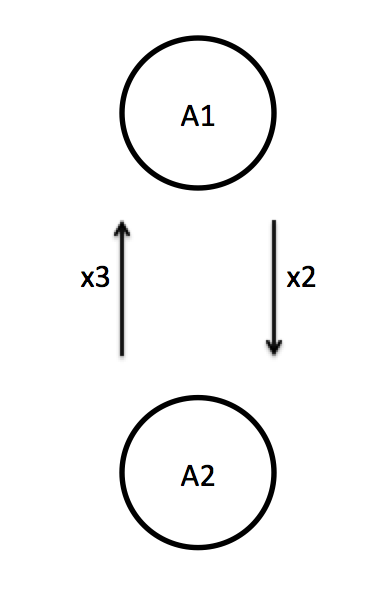
\includegraphics[scale=0.5]{simpletwofbex}
	\caption{\it Feedback loop between two algorithms A1 and A2, with each algorithm altering its output dependent on its input. A1s output is twice its input and A2s output is three times its input.}
	\label{fig:examplesimpletwofeedback}
\end{figure} 

This example was very simple, feedback loops can be much more complex, encompassing any number of entities, each of whom can have very complex algorithms for transforming their inputs. The financial markets are complex systems, so the entities involved in feedback loops will likely be interacting with a vast number of other entities, this can make detecting feedback loops very difficult.\\ %unsure about this sentence???? 
In the financial markets there can be a number of different objects involved in feedback loops such as, interbank loans or traded assets, this paper and the work that it is building on focus on the latter. A simple example of a feedback loop with traded assets is, a trader selling some of the assets due to falling market prices, causing the prices to be pushed down further and hence this trader to sell more of the asset to minimise their loses. This feedback loop can be considered malignant or a destabilising feedback loop, as it destabilise the market price. However not all feedback loops have a negative impact, some can be stabilising feedback loops due to a benign effect.\\      
Feedback loops can be present in a system in two ways, either they can be a constant fixture, a static feedback loop, or they can form and change, dynamic feedback loops. A static feedback loop is present in the system from the start whether this is intentional and known, or unintentional and unknown to the members of the system. Dynamic feedback loops my not be present at the start and can form and change over time, with new entities joining or leaving them, allowing them to increase or decrease in size or effect, to split or merge, or to disappear.\\
Feedback loops can operate across time, meaning that an event in the past can feedback to a present decision. Using the example of the seller selling their inventory to mitigate loss again, it can be seen that this loop operates over a time series, the seller sells some of their stock causing the price to go down then, however the process for this to happen and the seller to become aware of it is not, so at a later time the seller will see the drop in price and hence sell more stock. The time scale this example will happen over is quite smaller, however for a feedback loop containing a large number of entities the time scale on which the feedback occurs can be come significantly larger.\\
Due to the potential complexity of feedback loops both in construction and in time, they can be difficult to detect hence methods can be used to expose them. For static loops, forms of static analysis can be used such as, analysing initial setup, this is possible since the loops do not change through out time. Dynamic loops can be much harder to observe and analyses, an important aspect to detecting these loops is the interactions, messages sent between different entities within the system. Since the loops can evolve over time being able to track and analyse these messages over a time series is vitally important for the analysis of these loops, this time dependent analyse is called dynamic analyse.             




\subsection{Approach to Modelling the Financial Markets}

The aim of the work this paper is building on is to be able to create a model on which dynamic analyse of feedback loops can be done. More specifically this model aims to investigate feedback loops with in the market microstructure, looking at the fastest members of the system, High-Frequency Traders (HFTs).\\
HFTs are a subset of algorithmic traders who normally participate in the market as arbitrageurs or market makers, they invest in ultra-high speed technology allowing them to detect, analyses and react to market condition in nanoseconds \cite{hftinformation1}. This means HFTs can trade huge quantities of assets in very short time frames, with some estimates stating that 10-40\% of all trades where initiated by them during 2016 \cite{hftmarketparticipation}. For these reasons HFTs create fertile ground for the exploration of dynamic feedback loops.\\
To model the market microstructure and the HFTs interactions within it, the approach must be fine-grained and quantised in time.   

	
\subsubsection{Fine-Grained Microstructure Approach to Financial Markets} 

Due to the speed at which HFTs trade, the order in which events happen becomes very important. For example if two orders sent to an exchange are processed in the wrong order this could cause or destroy a feedback loop, hence making meaningful analyse impossible. Therefore a fine-grained approach which keeps track of both timings of interactions and ordering of messages between entities is required; modelling and storage of the precise order of message-passing and the messages is hence needed. To correctly order messages delays also have to be taken into account, these can be from constant elements such has how long it takes messages to pass through the cables between computers, or varying elements for instance the time taken for an exchange to process an order, which can increase with large traffic \cite{SECreport_delays}. Hence the approach to modelling a market in this detail requires the correct storage of message-passing, arrival order (that can be altered with different delays) and content.


\subsubsection{Discrete Time}

To model the market microstructure, message order and delays, time progression within the market must also be modelled. Though naively it is easy to assume that this time is continuous, this is not always the case and discrete time can sometimes be used. For example the market can be looked at in a long time horizon,  possibly for portfolios that only rebalance rarely, where the only time jumps of note are days, months or years, then time may progress discretely in chunks relating to the desired time step. Conversely very small time scales may be investigated, this is the case that pertains to HFTs market microstructure. Looking at very short time gaps it can be seen that the market actually operates at discrete intervals only progressing in very short time steps. This phenomenon is due to the use of electronic markets, since all markets that HFTs trade on are controlled by a computer they operate at a time set be the computers internal clock. Though computers can have a large amount of precision their clocks do not operate continuously and are in fact using discrete time prescribed by the change in voltage of an internal system clock, done by creating a square-wave oscillating voltage. Hence all trading on electronic markets, whether or not it started in continuous time, was sent by a human, will be curtailed into discrete time by the exchanges computers.\\
To a human this will still appear as a continuous time scale, however HFTs operate at such small time scales that this discrete time is comparable and therefore important to modelling them.          




\subsection{Agent Based Modelling}
%modeligng techinques, no model is right but some are useful 
%what is agent based modelign
%why was it chosen
%what are its benifits for this
%what are its down sides

%what is agent based modleing
%http://ieeexplore.ieee.org/abstract/document/5679168/


An agent-based model [REF] provides an attractive fit to modelling interaction dynamics in a System of Systems, since each component can be modelled by a separate agent or by a group of agents with varying levels of detail, with private communication within a group; furthermore, messaging and discrete time are handled naturally, and numerical solutions can be obtained for large problems that are analytically intractable.  However, we were initially wary of this approach because of the limitations that cause agent-based models to be not widely accepted by economists, as described for example by Gould et al [REF 2013] and Leombruni and Richiardi [REF].  For our purposes, the most important limitations appear to be:
?	Although each agent is fully specified, the model as a whole may lack a formal definition.
?	It can be difficult to track how a specified input parameter affects the output, and parameter-estimation may be achieved in a way that is not representative of all possible outcomes the model can produce. 
?	Finding a set of agent rules that produces a specific high-level behaviour provides no guarantee that it is the only set of rules to do so.
Leombruni and Richiardi [REF] resolved the first of these problems by providing a formal specification of an agent-based model in terms of a set of recurrence relations. This has the added advantage that the recurrence relations are easily understandable by non-programmers.  They also showed how to ameliorate the second problem by analysis of the sensitivity of outcomes to parameter selections.  The third problem remains, yet it is a problem shared by a wide range of models [REFS? HMMs?].





based model [REF] provides an attractive fit to a SoS, since each component system can be modelled by a separate agent or by a group of agents with private communication within a group (perhaps using a hierarchical agent-based model [REF]); furthermore, messaging and discrete time are handled naturally, and numerical solutions can be obtained for large problems that are analytically intractable.  However, we were initially wary of this approach because of the limitations that cause agent-based models to be not widely accepted by 


Agent based models (ABMs) are a kind of model which can be used for simulations. These simulations work by having a number of independent agents who each have their own behaviour interacting via messages sent between them, this system created by these interacting agents is the model. 
Because ABMs takes a radically different approach to the modelling of systems the difference equations, using a number of interacting agents each with their own behaviour that could be described as grouped difference equations instead of that large block of logic, which is inherent in difference equations, they can tackle some of the issues in a very different way. 
ABMs also have the ability to be run at a far faster pace then difference equations under the right circumstances, this is because they can be run in parallel computing architecture setups, allowing multiple calculations to be run simultaneously on different machines. 
They also tend to require far less recomputation then there difference equation counterparts due to the way, which they are set up and then run.
These features makes this method far more efficient for very large systems that otherwise could take a very large amount of computation time.  
ABMs operate in a step-by-step way making it very natural to create an ABM that has discrete time as each step. This means that at each step all the agents will send out their messages to other agents telling them their interactions at that particular time interval, this is a similar behaviour to how the real financial market operates. The exact time interval can be chosen by deciding upon the smallest time unit which will be used in the simulation and having everything else operate at integer multiples of this base time.


Discrete time is also used in coarse-grained models, where in different models an individual time step may represent an intraday period, a day, or perhaps a month (see for example [REF Huang et al] [REF Yan&Clack, etc]).  An important characteristic of discrete-time models is that each time step represents an equal amount of time; the extent of each time step may be defined (e.g. as a number of seconds, minutes, hours or days), though in some models (e.g. [REF Huang et al]) the extent is left unstated in the model and may then be instantiated in a numerical simulation. 


\subsubsection{Benefits} 
%it has denifits and downsides
%why it is used for this
%its ebnfits
	%computation speed
	%ease of thinking
	%store messages
\paragraph{Tracking Messages} 
\paragraph{Conceptually Easy to Understand} 
%look at the notes for chris course for more reasons

\subsection{InterDyne} 
%this is what has been made
%how it works
%what has it been used for already

%what is interdyne
%how does it work
%what do we want it to show

InterDyne is a simulator designed to look at interaction dynamics, these dynamics have been with in the financial sector but can in theory be any interacting system. 
This is an agent based simulator, this means that each component of an interacting system can be expressed as an agent, in the case of a financial system agents could be individual traders. Interactions between the agents can then be defined, these could be messages sent between a trader and an exchange for placing an order. 
Once the simulator is set up in this way it can run through steps, at each step the interactions between the agents are passed and each agents response to the interaction is processed, these steps can represent discrete time.   
InterDyne adds no direct mechanism that would force the system as a whole to exhibit any specific behaviour, any emergent behaviour experienced by the system is a result of the interaction dynamics only.\\ 
A more complete way of labelling InterDyne would be as; a simulator used to investigate interaction dynamics and feedback effects in non-smooth complex systems~\cite{Chris_webPage}.





from book 
Interdyne is a simulator that is designed to allow for exploration of interaction dynamics and feedback effects in non-smooth complex systems, though this is a general purpose simulator that can be used in a variety of fields its setup makes it especially sorted to modelling the financial system that has been described above.  Below the aspects of Interdyne will be explained showing how it satisfies the criteria needed to model the finical markets. 
Like other agent-based models InterDyne operates in discrete-time, this discrete-time can be left without a proper definition in terms of real time, this is normally done in experiments that are interested purely in general behaviour of a system. Though real time mapping is easily achievable by simply taking the smallest time step that will need to be used with in a simulation and then mapping all time steps as a integer multiple of it.  
Being an agent-based model InterDyne allows communication between agents as the only form of interaction. This communication can be done in a one-to-one or one-to-many format, allowing for agents to send out broadcast messages which can be read by all other agents or send private correspondents that can only be seen by one other agent. Both of these messaging types are needed in modelling the markets, for example an exchange would send out a broadcast message to all members updating them on the order book, where as a trader would send a private message to a exchange when they want to place a order. 
To allow a full understanding and the precise use of these messages, a communication topology can be defined within InterDyne. This topology will defined the interaction paths between agents and as such which communication routes are possible and which are not. This topology takes the form of a directed graph (allowing on agent to trader with another but not vice versa) with the agents acting as the nodes and the communication paths acting as the edges. 
As with most real systems messages are not passed instantaneously and as such InterDyne supports the use of information delays, these delays are unique to each interaction path between agents, as defined in the communication topology.  These delays apply to any messages using these interaction paths, whether the message is defined as a one-to-one or a one-to-many.  





To allow InterDyne to model a system of systems and not just a flat system each agent can be modelled with differing levels of detail. This can take the form of having a simple agent generating outputs dependent on a statistical distribution, interacting with a trading algorithm, which contains a great amount of detail and complexity. An agent can also contain another InterDyne simulation as its internal structure, giving a true system of systems depth to the model.
The InterDyne simulator as a whole is built to be deterministic, meaning that any run of an experiment that contains the same inputs will always give the same output. This behaviour is very beneficial for analysis of low-level interactions that cause complex behaviour as it allows for a more detailed examination of the causal pathways that cause this behaviour. Though InterDyne is designed to be deterministic, non-determinism can be added to a simulation in two different ways. Either non-deterministic elements can be added directly to the agents (such as use of stochastic calculus to calculate some aspect of placing orders), or for an agent that receives multiple messages in one time step (such as an exchange receiving orders from a large number of traders) these messages can be sorted randomly (alternatively they can be sorted according to the senders identity).  This random sorting is in actuality pseudo-randomly, as for every run of the simulation the same random order will be reached, this can be changed to being truly random (or as much as a computer can allow) using a different seed for each run of the simulation.


\subsubsection{Harness} 
%used to connect the agents and monitor the interactions


\subsection{Example}
%examples of real world feedbakc loops






Day and Huang [Day, R. And Huang, W., ?Bulls, Bears and Market Sheep?, Jourmal of Economic Behaviour and Organisation, 1990] for example have demonstrated how interactions between two simple but different trading strategies and a market-maker can cause complex emergent features of stock market prices such as alternating periods of rising (?bull market?) and falling (?bear market?) with sudden switching between the two at irregular intervals. Further, Lyons [Lyons, R.K. ?A Simultaneous Trade Model of the Foreign Exchange Hot Potato?, Journal of International Economics 42 (1997) 275?298] has shown how a feedback loop can emerge between foreign exchange dealers, causing them to repeatedly transfer inventory between themselves.  Yet these are simple models of interaction.  Our aim is to develop a framework for modelling and analysing more complex emergent behaviour that arises from the dynamics of interaction, and in the context of our case study to analyse behaviour that may increase risk to the stability of the financial markets.

\subsubsection{Hot Potato} 
%what is hot potato
%fx market

%this is a dynamic feedback loop
%how is it caused 
%when has it happened 

%what is a hft (probably need a subsectuion on this)
	%how do they work
	%what do they do
	%market makers
	%inventory limits
	%why do simple versions of them still work

To understand the hot potato effect one must first know that High Frequency Traders have strict inventory limits and that when these limits are passed they are said to be in a ``panic state''. During a panic state the traders will issue large sell market orders to reduce their inventories back into their ideal trading regions. A High Frequency Trader can go into a panic state when it unintentionally buys more inventory then intended, which can happen due to information delays in the confirmation of purchases. It is thought that in the flash crash High Frequency Trades panicked when buying from a mutual fund who issued an unusually large sell order. Once one High Frequency Trader has panicked its now sold inventory can be bought by another trader who, again because of information delay, surpass their inventory limits and in turn panics. This processes can continue indefinitely depending on the system and is known as the hot potato effect as the inventory is constantly passed around and not retained by an one trader~\cite{Elias_Paper}. This feedback effect has been shown, in the InterDyne simulator, to create instabilities in market prices and even lead to crashes~\cite{DynamicCoupling_Chris}.   






\subsubsection{Flash Crash}
%lob version of hot potato
 
%what is the flash crash
%when have they happned 
%other theories to why they happen?
%what we think causes them
	%emergence from feedback loops in hfts
%why they are important
A flash crash is defined as a quick drop and then recovery in securities prices, with the most infamous  crash occurring on the 6th of May 2010 and lasting for around 20 minutes in which time almost one trillion dollars of market value was lost~\cite{Vikram_Paper}.\\
There is no consensus on the exact cause of the flash crash, however a number of theories exist. The theory that InterDyne models is that the flash crash was caused by an interaction effect between High Frequency Trader Market Makers, known as the hot potato effect~\cite{Elias_Paper}. 



There are numerous examples of emergent behaviour in the financial markets caused by interaction dynamics within the SoS, here we will look at how the US markets ?Flash Crash? of May 6th 2010 [CFTC-SEC, 2010. ?Findings regarding the market events of May 6, 2010?] may have been caused by these interaction dynamics. 
The term ?Flash Crash? here is used to describe an event within a financial market where the price of commodities plummets extremely quickly before rapidly rebounding. This kind of behaviour tends to go hand and hand with commodities becoming disconnected from their fundamental value, such as stocks for companies trading at far lower prices despite the fact that mothering has change about the company in question.
The crash in question occurred within the E-mini S&P 500 market, EXPLAIN WHAT THIS MARKET IS, lasting approximately thirty minutes [REF] with the prices for some stocks falling as low as a penny a share [REF].
FIGURE OF FLASH CRASH??? 
There has been a large amount of speculation about the cause of this crash with blame levelled at a large sale by a mutual fund, spoofing by a independent trader and the hot potato effect between High Frequency Traders (HFTs), it is the later that we are interested in here.
HFTs are algorithmic traders who use equipment that allows them to operate at nanosecond speeds [REF], this means huge amounts of trading can occur between HFTs before a human can process what has happened.  Not sure how to phrase this but want to say that a lot can go wrong before a human realises 
HFTs often operate as a Market Maker, these are entities that both buy and sell with the market under a set of rules, such as having to always have a bid and ask on the order book, they are then rewarded by having discounts applied to their trades. Market Makers make their profit of the difference in price between buying and selling assets and not of the fluctuation in price of an asset over time. They would not buy assets with the aim of selling them in a few days as they think the price would increase, instead they buy and sell the assets normally within a few milliseconds. As such having a large inventory of any asset is considered to be risky by the Market Maker and they will normally have thresholds on their stock, if these thresholds are passed, they have more stock then they want, they will enter an aggressive selling phase, quickly reducing their stock back below their thresholds. When this occurs the HFT is said to be in a panic state, the inventory at which this panic state occurs can be dynamic, changing demanding on the perceived risk within the market and how the Market Maker is trying to preform. 
Since HFTs can place orders so quickly and make their profit of buying and selling they will normally have orders near or at the touch, the best bid and ask. This means that if you trade on the market you are likely to execute your trade with a market maker first SAY WHAT PERCENTAGE OF TRADES THE MARKET MAKERS ARE RESPONSIBLE FOR [REF]. This means that if a Market Maker goes into panic it is likely to sell its stock to another Market Maker; this creates links between the Market Makers as they will buy and sell to each other during panic states.  
There are a number of methods used for exiting a panic state, enough inventory can be solid to bring the Market Maker back to exactly its limit, more can be solid to bring it below its limit by a set amount or all the inventory can be solid to reduce the risk to the Market Maker to zero. Each of these different options changes how much stock will be passed on to another Market Maker during the panic state.
The question then arises, what happens if the Market Maker who buys this excesses stock is already near its inventory limit? In this case the receiving Market Maker can also enter panic, causing it to sell its inventory back to the market. As can be imagined in the right market conditions, this inventory can be picked up by another Market Maker who is also close to their limit and hence the processes can continue. If this inventory passing between the Market Makers forms a feed bank loop, where the initial Market Maker receives the stock again before selling it on for a second time, it can be said that ?Hot Potato? effect is occurring, this is simply the processes of passing inventory around traders in a loop.    
There are a number of reason a Market Maker could be near its limits or go into panic, it could be already near its limits and then be forced to buy more inventory by the exchange rules. It could dynamically shift its risk limits changing its inventory boundaries causing it to go into panic or at least approach its limits or it could make a number of assumptions about its sell orders which may be incorrect. 
A reason assumption are made is because of time delays with in the system. 






\section {Description and analysis of the problem} 
%simulations in itnerduyne not fully excepted by exconimists


%this model is not fully excepted by econimists
%why this is so
%a method to fix this

\subsection{Why Agent Based Modelling is not enough}
%

%why agent based modeling is not perfect for being excepted
%one to many relationship
%an alternative differnce equations

\subsubsection{One-to-Many Problem}
\subsubsection{Semantics of the System} 
\subsubsection{Inverse Function Problem?} 

\subsection{Difference equations} 
%what are difference equations
%how do they work
%why are they more easily excepted

Leombruni and Richiardi [REF] have shown how a discrete-time agent-based model of the dynamic microstructure of financial markets can be expressed as a set of recurrence relations.  In their formulation, each agent is well described by a state variable given by xi,t where i is the agent identity (i ? 1, ... , n) LC- in a n agent problem and t is time, and where each xi,t+1  

 \subsubsection{Benefits and Problems} 
 %other benfitis and down sides of them
 
 \subsubsection{Lack of Visualisation} 
%but they won?t be able to ?see? the emergent behaviour with running the simulator ?

\subsubsection{Optimisation Problems} 
% but generally we can?t directly ?run? these equations because for any reasonable-sized system there will be too much recomputation (we get the same problem with dynamic optimisation problems!)
%there are ways to cache intermediate results, but they ain?t pretty

\subsection{Two Views Approach} 
%My solutions, two view
%what is two views
%its benifits
%how it will solve the problem
%look at refrence in book chapter relating ABM to difference equations


from book
As can be seen in the previous sections there is no one perfect method for modelling the interaction dynamics and emergent behaviour with in the financial system. Due to the nature of this system it has been concluded that the two most useful models are difference equations and agent based models, however these two methods give very different views of the system making it impossible to be able to claim that one single method is more useful then the other in all cases. From this problem a natural question arises: is it possible to combine these two methods and hence reap the benefits that they both have, off setting the negatives of each other? The answer to this question we call the two-views approach, this is a way of combining both methods to tackle the same problem. The way in which we combine these two methods is to first define the problem using difference equations, allowing the benefits of this method to be used such as defining the semantics of the problem. Once the problem has been defined it is converted into an agent-based model using series of correctness preserving transformations. This allows the now agent-based version of this problem to still contain the same information that was present in its difference equation form, while now also now being able to be modelled with the benefits of the agent-based model.      
This method is specialised and a custom language for difference equations has been defined, that is an expansion of lambda calculus. This language has been defined in such a way that it can be used to express a problem so that the function of the agent-based model can still be fully utilised. The agent-based language that is used is designed to contain all the aspects need for expressing the financial markets: message passing, communication delays and interaction topology definition. We call this bespoke agent-based model Interdyne. 

\section{Converter} 
%how I will create the two views
%what the converter is meant to do


\subsection{New Language}
%first step is to create a language which can be used by a user to create a propram as difference equations
%language has to be simple enough that a non computer scientist/econimist can use, but must still be able to contain all the information required for the program
%programs wirtten in this language will be parsed into lexemes and then converted into a numeric type (?) which will be used to transfer this into lambda calcus and an ABM model

\subsubsection{Syntax/Grammer}
%what the new language looks like 
%what each bit means
%what is allowed to be written
%how to write certain things
%how is it user friendly
%why this was choosen, for example easier to convert to lambda calcualse 
\subsubsection{Parser}
%explain what the parser is and how it works, in preparing these files for transfermation
\subsubsection{Examples}
%examples on how to use the grammar
\paragraph{Simple Example}
%a very simple example on the use of the grammar
\paragraph{Complex Example}
%what I have actually done maybe?





\section{Conclusion}
\subsection{Further Work}

 
\section{Appendix}

\subsection{Appendix 1} %\label{Appendix_1}
%\lstinputlisting[language=C++]{AllCode_functions.cpp}


\addcontentsline{toc}{section}{References}
\bibliographystyle{unsrt}
\bibliography{MRes_Dissertation}







     
\end{document}










